\documentclass[12pt,a4paper,openright]{report}

\usepackage[italian]{babel}
\usepackage{newlfont}
\usepackage{parskip}
\usepackage[utf8]{inputenc}
\usepackage{fancyhdr}
\usepackage{hyperref}
\usepackage{geometry}
\usepackage{babelbib}
\usepackage{minted}
\usepackage{graphicx}
\usepackage{amsmath}
\usepackage[font=footnotesize]{caption}

%serve solo per il frontespizio
\textwidth=455pt \oddsidemargin=0pt

% Direttive fancyhdr, si può fare riferimento al layout:
% {lhead}   {chead}   {rhead}
%        <Page content>
% {lfoot}   {cfoot}   {rfoot}

\pagestyle{fancy}%\addtolength{\headwidth}{20pt}
\renewcommand{\chaptermark}[1]{\markboth{\thechapter.\ #1}{}}
\renewcommand{\sectionmark}[1]{\markright{\thesection \ #1}{}}
\rhead[\fancyplain{}{\bfseries\leftmark}]{\fancyplain{}{\bfseries\thepage}}
\lhead{\leftmark}
\rhead{\thepage}
\cfoot{}

\linespread{1.2}

\begin{document}

%frontespizio
% Frontespizio reperito da: https://corsi.unibo.it/magistrale/ScienzeInternet/tesi-in-latex
% e liberamente modificato da Guglielmo Palaferri


%\documentclass[12pt,a4paper]{report}
%\usepackage[italian]{babel}
%\usepackage{newlfont}
%
%\begin{document}



\begin{titlepage}
\begin{center}
    

{{\Large{\textsc{Alma Mater Studiorum $\cdot$ Universit\`a di
Bologna}}}} \rule[0.1cm]{15.8cm}{0.1mm}
\rule[0.5cm]{15.8cm}{0.6mm}
{\small{\bf SCUOLA DI INGEGNERIA E ARCHITETTURA\\
Corso di Laurea in Ingegneria Informatica }}
\end{center}
\vspace{35mm}
\begin{center}
{\LARGE{\bf Porting di un algoritmo per la stima del flusso ottico su smartphone Android}}\\
\end{center}
\vspace{50mm}
\par
\noindent
\begin{minipage}[t]{0.47\textwidth}
{\large{\bf Relatore:\\
Prof.\\
STEFANO MATTOCCIA}}
\end{minipage}
\hfill
\begin{minipage}[t]{0.47\textwidth}\raggedleft
{\large{\bf Candidato:\\
GUGLIELMO PALAFERRI}}
\end{minipage}
\vspace{20mm}
\begin{center}
{\large{\bf Appello II\\%inserire il numero della sessione in cui ci si laurea
Anno Accademico 2020-2021}}%inserire l'anno accademico a cui si è iscritti
\end{center}
\end{titlepage}

%\end{document}

\newpage
%\clearpage{\pagestyle{empty}\cleardoublepage}

\pagenumbering{arabic}

%il textwidth=455pt serve per il frontespizio, è troppo grande per il testo
\newgeometry{textwidth=426pt}

\shipout\null
\tableofcontents

%\lhead{\leftmark}
%\rhead{\thepage}
\chapter{Introduzione}
%\addcontentsline{toc}{chapter}{Introduzione}
%\lhead{INTRODUZIONE}

Il monitoraggio costante della velocità di fiumi e correnti d'acqua può assumere notevole importanza sia nello studio di 
fenomeni idrologici puramente naturali, sia nella progettazione di opere ingegneristiche strettamente legate ad un 
particolare flusso d'acqua. Ad esempio, può aiutare ad analizzare e rilevare fenomeni come le inondazioni (specie gli 
avvenimenti improvvisi, che destano particolare attenzione), così come anche il trasporto di sedimenti o 
l'erosione delle rocce.

Come evidenziato in \cite{rs10122010}, molte delle tecniche tradizionali utilizzate per l'osservazione di un flusso idrico, tuttavia, non garantiscono 
grande efficienza e presentano costi elevati: spesso è richiesta la presenza di personale specializzato per la 
manutenzione di dispositivi complessi.\\ %citazione a paper remote sensing
Una soluzione che preveda invece l'installazione di apparecchi ottici, e basi quindi il monitoraggio sull'elaborazione di
immagini, può consentire di abbattere notevolmente i costi e di distribuire il sistema di osservazione ottenendo quindi 
maggiore resistenza ai guasti.%inserire immagine di esempio applicazione OTV.

\begin{figure}[h!]
    \begin{center}
        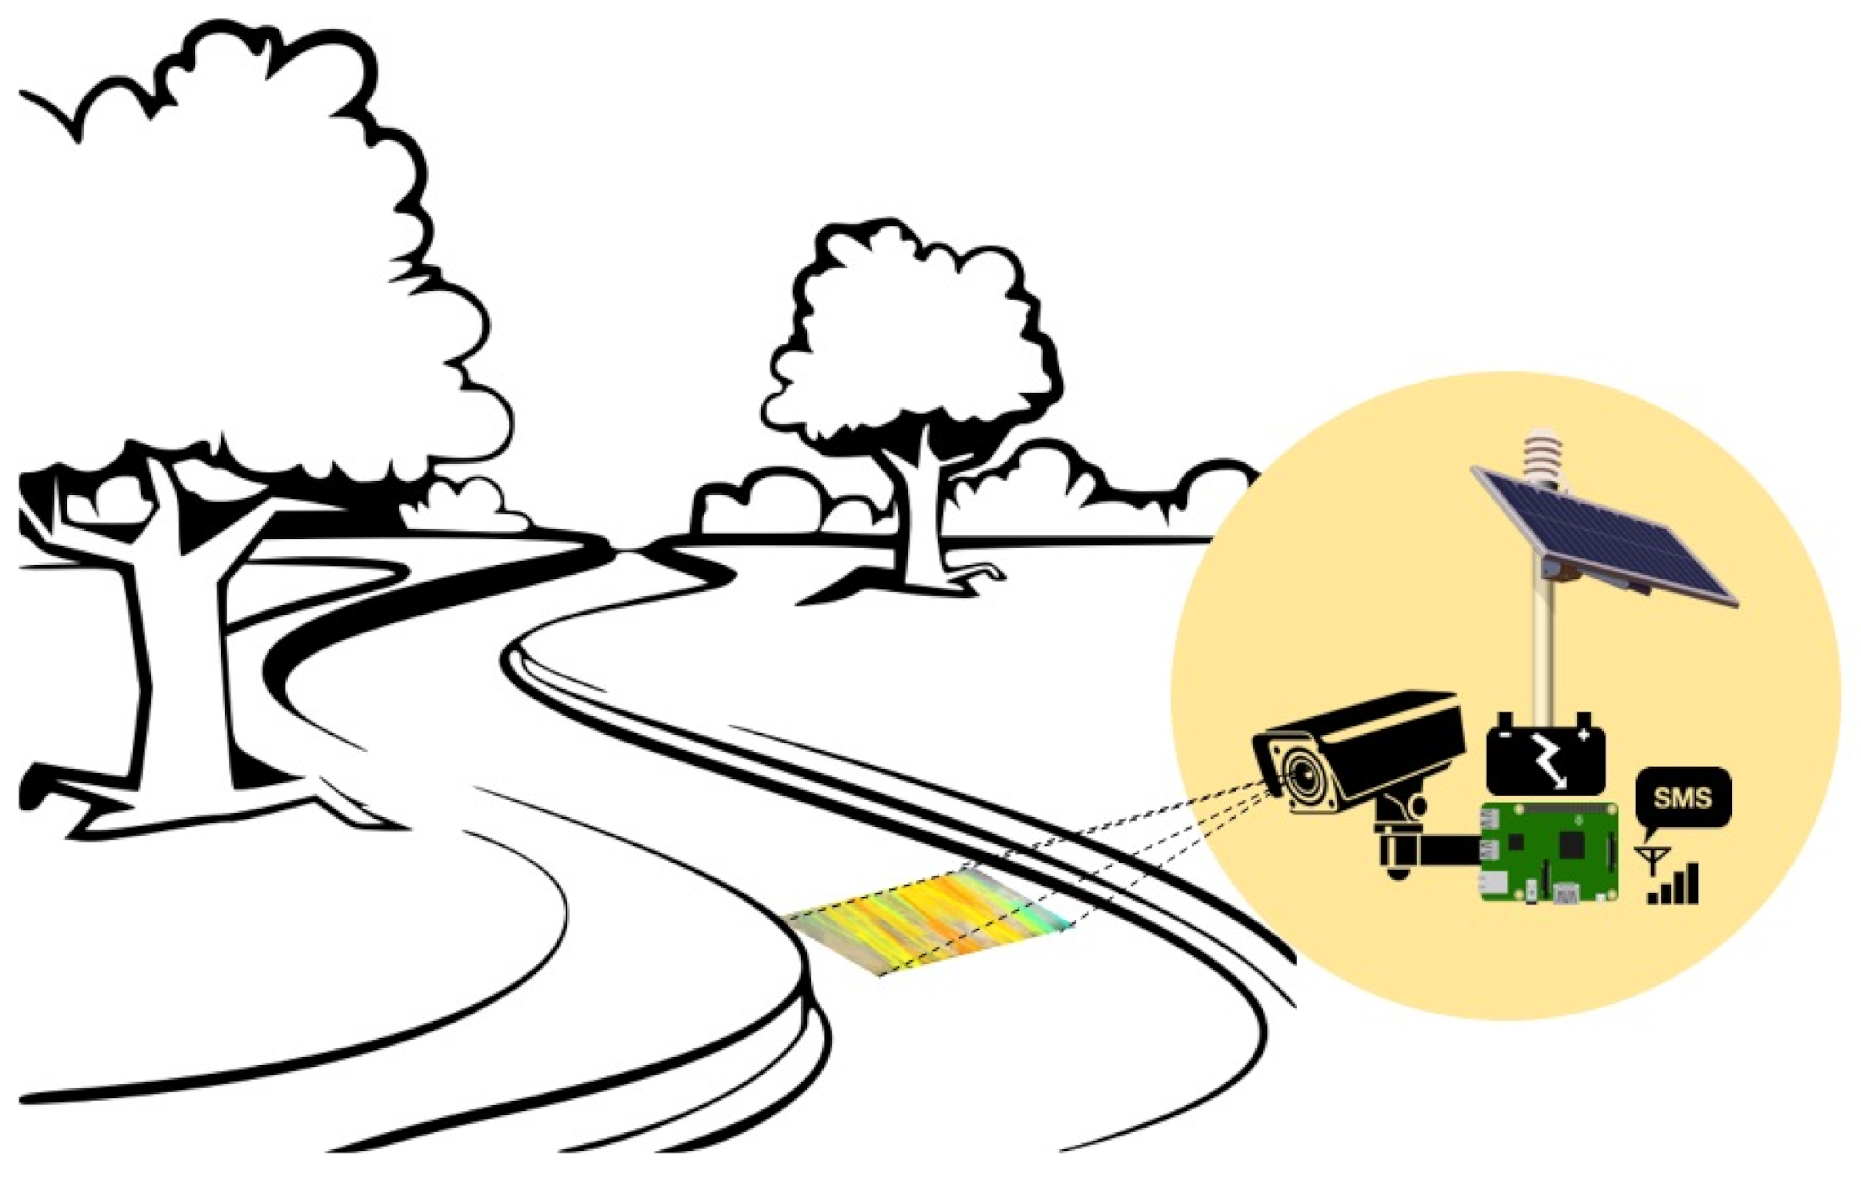
\includegraphics[scale=0.2]{img/otv_real_use.png}
        \caption{Esempio di installazione di un dispositivo embedded basato sull'elaborazione ottica}
    \end{center}
\end{figure}

È proprio questo un caso di utilizzo di \textbf{OTV} (\textit{Optical Tracking Velocimetry}), una tecnica che fa uso di 
particolari algoritmi di computer vision (in particolare l'algoritmo di \textit{Lucas-Kanade}, utilizzato per la stima 
del flusso ottico) per tracciare le traiettorie e le velocità del flusso d'acqua a partire da una serie di immagini. 
Il tracciamento viene svolto grazie al riconoscimento di particelle quali detriti e altri residui e al confronto di fotogrammi 
consecutivi.

Il metodo OTV è pensato per essere applicato a dispositivi di elaborazione a basso costo e di dimensioni contenute: questi
sarebbero posizionati lungo corsi d'acqua in aree geografiche remote. I dati poi raccolti da questi dispositivi potranno essere
spediti (tramite meccanismi semplici come l'invio di SMS) ad un sistema di raccolta dati centralizzato.
Va da sé dunque che l'ottimizzazione dei consumi energetici dei dispositivi costituisca un punto cruciale per la 
realizzabilità di un tale sistema di monitoraggio. Questo tema verrà preso in considerazione e rappresenta uno dei punti
principali degli studi finora condotti sull'argomento.

\begin{figure}[h!]
    \begin{center}
        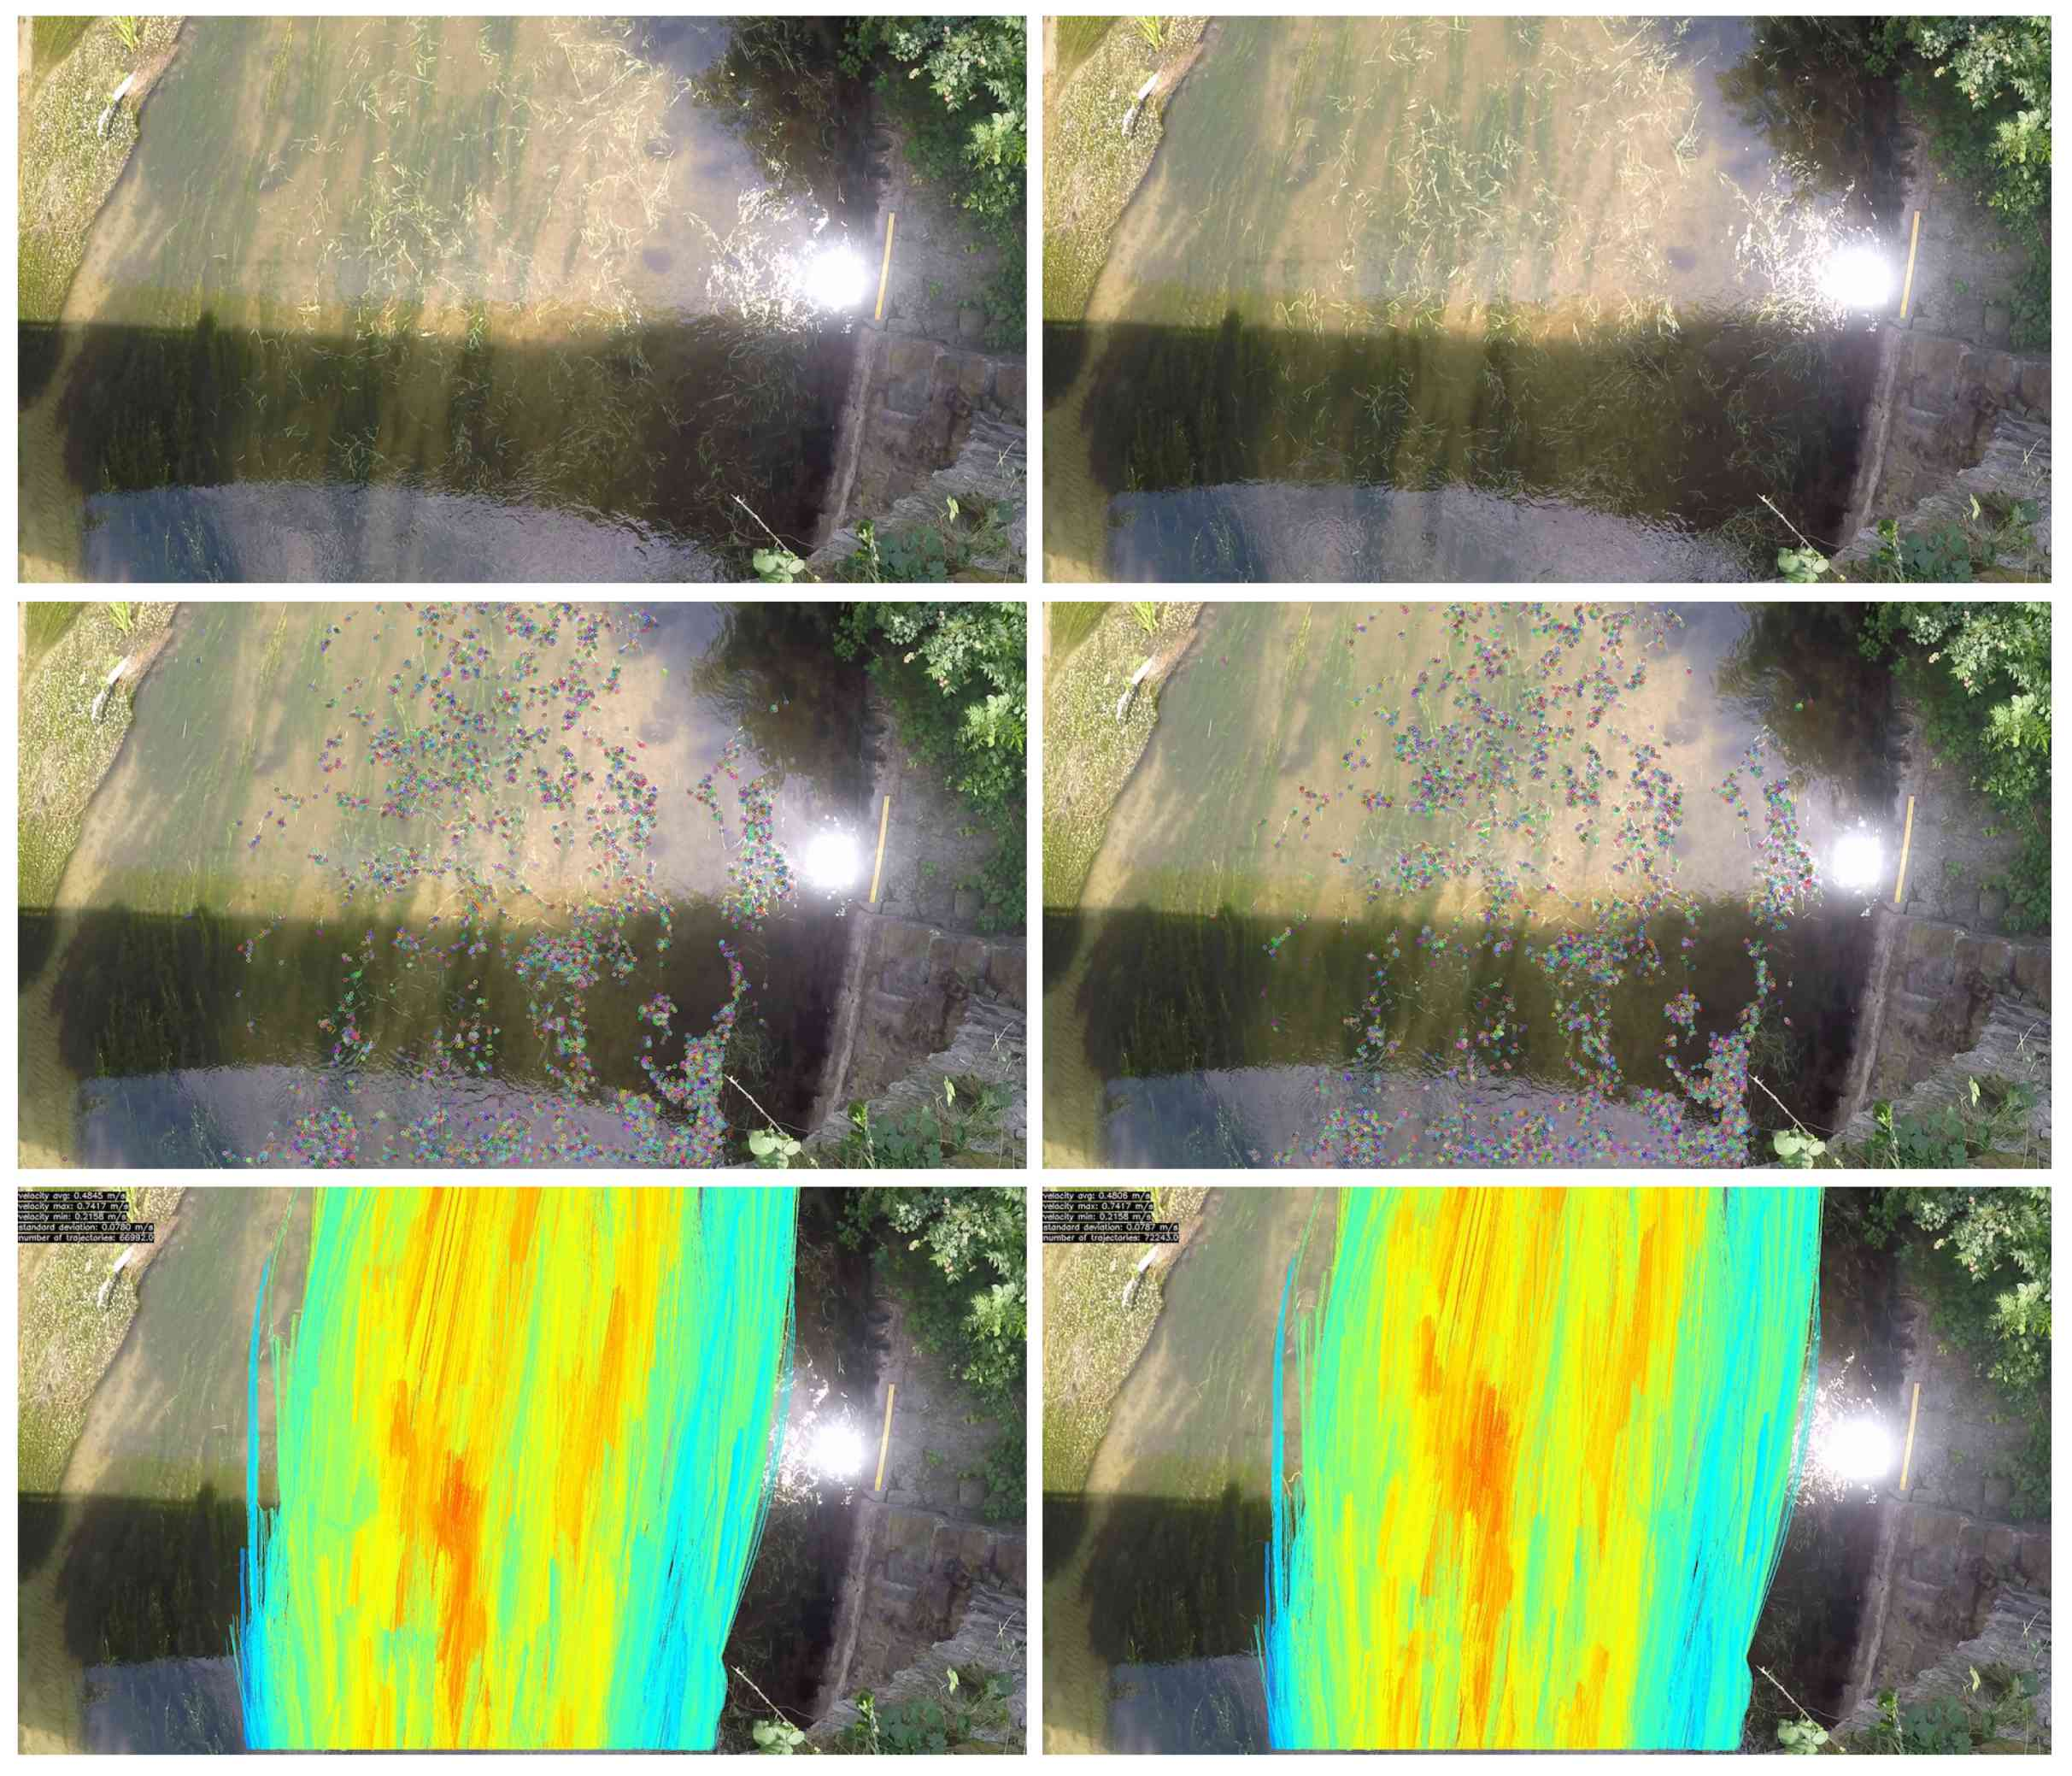
\includegraphics[scale=0.13]{img/sequenze_video_otv.png}
        \caption{Sequenze video ottenute con OTV: le linee tracciate rappresentano le traiettorie riconosciute, colorazioni
        più calde indicano velocità maggiori}
    \end{center}
\end{figure}

L'algoritmo è stato inizialmente testato su dispositivi della famiglia \textit{Raspberry}, per via delle loro dimensioni molto
contenute e in generale per le funzionalità da essi offerte, molto coerenti con i requisiti del progetto. Le analisi \cite{app11157027} 
hanno riportato ottimi risultati dal punto di vista dei consumi energetici in particolare dei modelli Raspberry Pi 3B e 4. 

Altri dispositivi con buone potenzialità e con un profilo che si presti bene al contesto di utilizzo sono gli \textbf{smartphone},
con particolare riferimento a quelli basati su sistema operativo \textbf{Android}. L'utilizzo di tali dispositivi richiede ovviamente
una seppur minima quantità di modifiche rispetto al deployment effettuato su Raspberry, ed è proprio questo il tema centrale
del seguente documento.

Nei prossimi capitoli si procede quindi --- dopo aver introdotto qualche informazione necessaria su OTV --- a descrivere 
la realizzazione di un'applicazione per smartphone Android che adatti l'implementazione in C++ di OTV (disponibile su GitHub al link 
\cite{otvgit}) e i risultati in termini di prestazioni e consumi energetici che ne sono conseguiti.




\clearpage{\pagestyle{empty}\cleardoublepage}

%\rhead[\fancyplain{}{\bfseries\leftmark}]{\fancyplain{}{\bfseries\thepage}}
%\lhead[\fancyplain{}{\bfseries\thepage}]{\fancyplain{}{\bfseries
%INDICE}}
%\clearpage{\pagestyle{empty}\cleardoublepage}

%++++++++++++
\shipout\null
\stepcounter{page}

\chapter{OTV}
\section{Contesto di utilizzo}

Come già brevemente descritto, OTV prevede un deployment su dispositivi di dimensioni ridotte e autosufficienti dal punto di
vista energetico. In particolare, la configurazione testata su Raspberry \cite{app11157027} introduceva i seguenti componenti:
\begin{itemize}
    \item Raspberry Pi 3B/4 per l'elaborazione
    \item Panello solare 6 W (PiJuice Solar Panel) per sostenere i consumi energetici
    \item Batteria esterna (PiJuice Hat) per fornire alimentazione
\end{itemize}
 Una simile configurazione verrebbe usata con smartphone, salvo ovviamente l'utilizzo di una batteria 
aggiuntiva.

\begin{figure}[h!]
    \begin{center}
        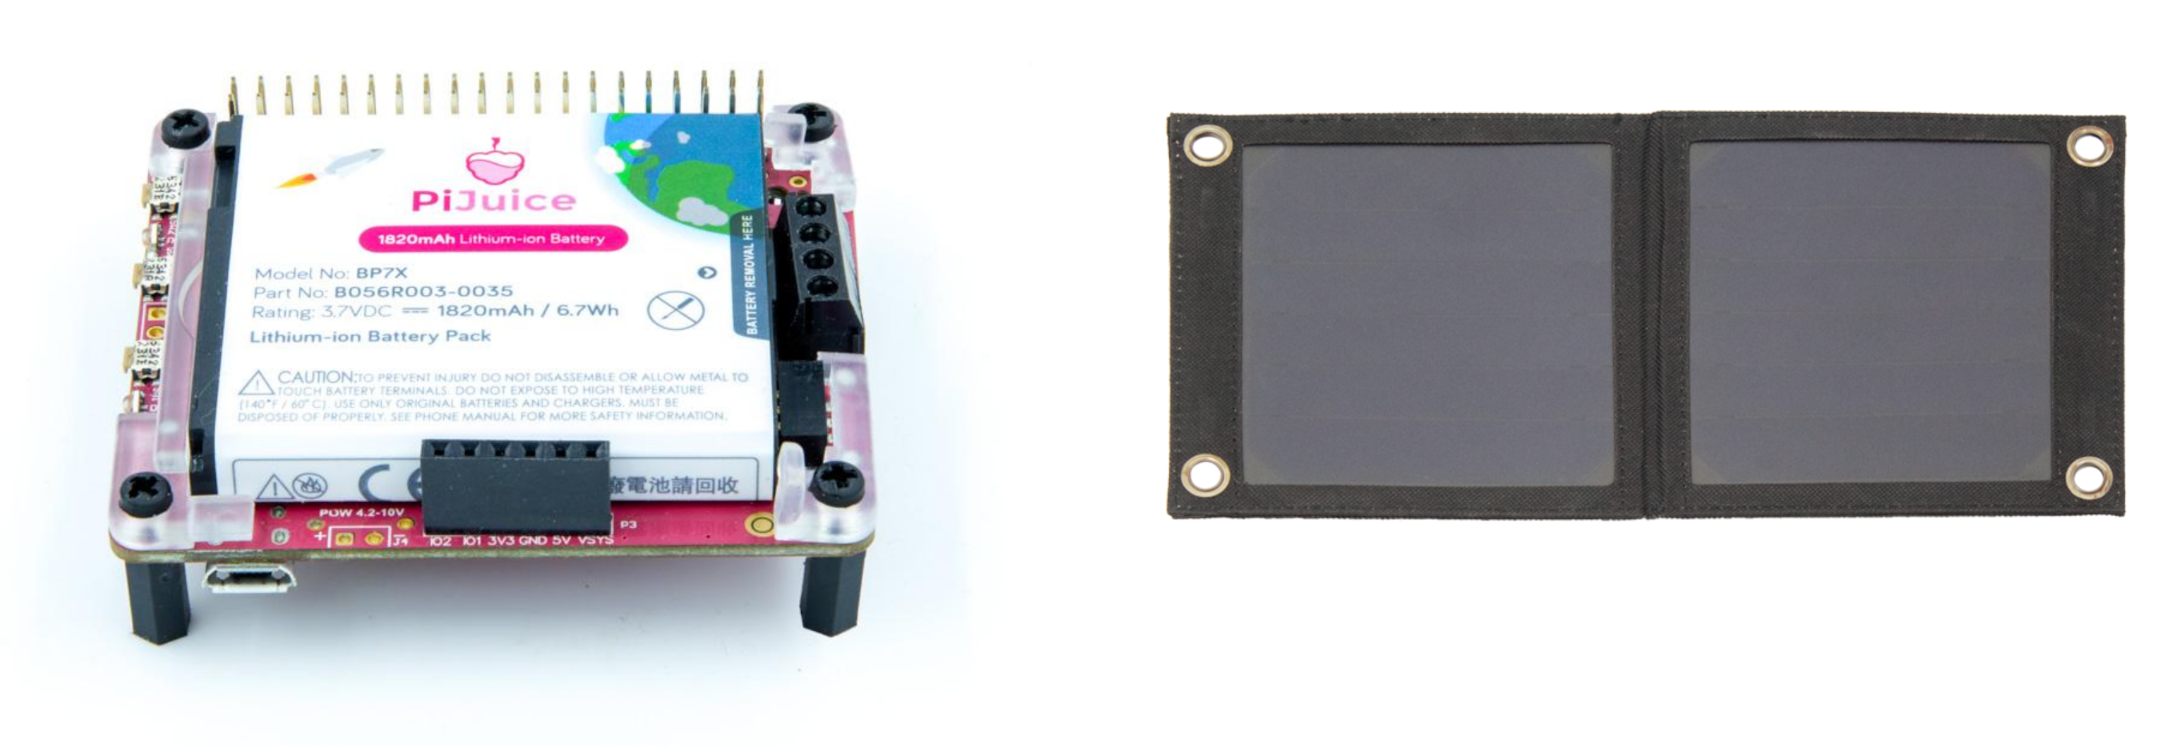
\includegraphics[scale=0.15]{img/pijuice.png}
        \caption{Esempio di deployment del dispositivo su Raspberry Pi}
    \end{center}
\end{figure}

\section{Ciclo di funzionamento}
\label{sec:ciclo}

Il dispositivo Android così composto, una volta accuratamente posizionato ed avviato, dovrebbe eseguire \emph{quattro} misurazioni 
della velocità dell'acqua ogni ora, risultando quindi a regime in un ciclo di funzionamento periodico della durata di 15 minuti.

Sebbene la misurazione mediante l'algoritmo OTV sia svolta sul momento, non viene effettuata sulle immagini direttamente ricevute
e lette in input dalla telecamera: il video acquisito necessita di una fase preliminare che prepari le immagini per essere elaborate.
Questo viene fatto, tra le altre cose, per consentire di scegliere un settaggio particolare (ad esempio, selezionare una 
risoluzione diversa rispetto al video originale), utile successivamente al fine di ottimizzare l'elaborazione.

Il ciclo di funzionamento si articola quindi in questo modo:
\begin{enumerate}
    \item Fase di \textbf{acquisizione}: le immagini vengono acquisite dalla telecamera. Questa fase ha una durata fissa e dipende
    dalla lunghezza del video che si vuole analizzare: tipicamente 20 secondi.
    \item Fase di \textbf{estrazione} dei frame: a partire dal video acquisito, si estraggono i fotogrammi che lo compongono a seconda
    della configurazione scelta, in particolare è possibile specificare la risoluzione desiderata tra:
    \begin{itemize}
        \item Full Resolution (\textbf{F}): Risoluzione originale
        \item Half Resolution (\textbf{H}): Risoluzione dimezzata
        \item Quarter Resolution (\textbf{Q}): Risoluzione 1/4 dell'originale
    \end{itemize}
    \item Fase di \textbf{elaborazione} (OTV): a questo punto le immagini estratte vengono effettivamente elaborate utilizzando
    OTV. Questa fase è cruciale dal punto di vista dei consumi in quanto è quella che può variare maggiormente a seconda della
    configurazione usata e delle ottimizzazioni implementate. È bene quindi analizzarla di conseguenza.
    \item Fase di \textbf{idle}: una volta conclusa l'elaborazione (ed eventualmente spediti i dati rilevati) segue un periodo di stand-by,
    in cui si attende il tempo necessario prima della prossima rilevazione. Anche questa fase è molto importante per determinare
    i consumi energetici del processo: se il dispositivo dovesse disporre di una modalità di risparmio energetico, 
    l'energia utilizzata potrebbe diminuire drasticamente.
\end{enumerate}

Le fasi su cui è possibile effettivamente lavorare per ottenere risultati migliori sono quelle di elaborazione (in modo particolare)
e di idle.


Prima di introdurre i vari livelli di ottimizzazione, va intanto fatto notare che la specifica implementazione di OTV presa in
caso è basata sulla libreria open-source di computer vision \textbf{OpenCV}.\\
OpenCV fornisce un framework per la creazione di applicazioni legate alla computer vision e implementa una vasta gamma di
algoritmi, tra cui l'algoritmo di Lucas-Kanade utilizzato da OTV già menzionato.\\
L'utilizzo di OpenCV prescrive una serie di passaggi di installazione che variano in base all'ambiente di sviluppo e che
--- nel caso specifico di Android --- verranno analizzati nel successivo capitolo.

\section{Ottimizzazioni}
\label{sec:ottim}

Le ottimizzazioni applicabili ad OTV analizzate in \cite{rs12122047} consistono in una serie di tecniche e meccanismi che
possano contribuire ad aumentare l'efficienza energetica del sistema. %e in generale ad abbassarne i consumi. 
Tra queste, possiamo distinguere quelle legate al \textbf{software} e quelle invece a livello \textbf{hardware} 
(ad esempio, l'utilizzo di istruzioni particolari).

Le ottimizzazioni software consistono essenzialmente nella configurazione del dispositivo in modo ad esempio
da disattivare le opzioni software che risultino superflue (Wi-Fi, Bluetooth ecc.). Si parla di ottimizzazioni derivanti dal
sistema operativo utilizzato e dunque dipendenti dal dispositivo in questione. Si vedranno ottimizzazioni di questo tipo
esclusive al sistema Android.

Per quanto riguarda le ottimizzazioni software, una di queste è risultata particolarmente efficiente nei test effettuati
su Raspberry mostrati in \cite{app11157027}: l'elaborazione in \textbf{scala di grigi} (o \textbf{monocromatica}). 
Non si tratta di una configurazione a livello di sistema operativo bensì di una piccola modifica al codice di OTV: 
i fotogrammi precedentemente estratti vengono acquisiti --- mediante le API di OpenCV --- come immagini monocromatiche invece 
che a colori. Questo passaggio non comporta  risultati particolarmente diversi (in termini di velocità e numero di 
traiettorie rilevate) ma consente di ottenere un notevole guadagno in termini di prestazioni. Questo deriva dal fatto che le 
immagini in scala di grigi sono composte da un singolo canale, a differenza delle immagini a colori rappresentate invece da 
tre canali (Rosso, Verde, Blu).

\subsection{Ottimizzazioni hardware}

Nel caso delle ottimizzazioni hardware, si parla di particolari metodi che introducono differenti modelli di esecuzione
a livello di processore, facendo leva specialmente sulla parallelizzazione delle istruzioni. Questo, oltre agli ovvi vantaggi
in termini di performance, può portare ad una maggiore efficienza in termini di consumi.
Si delineano tre possibilità principali, eventualmente sovrapponibili, focalizzate su aspetti e modalità diverse di 
parallelizzazione:
\begin{itemize}
    \item Esecuzione multi-core mediante \textbf{OpenMP} o \textbf{TBB}. 
    \item Esecuzione di istruzioni \textbf{SIMD} tramite \textbf{NEON}
    \item Esecuzione su \textbf{GPU} mediante la libreria \textbf{OpenCL}
\end{itemize}

\begin{figure}[h!]
    \begin{center}
        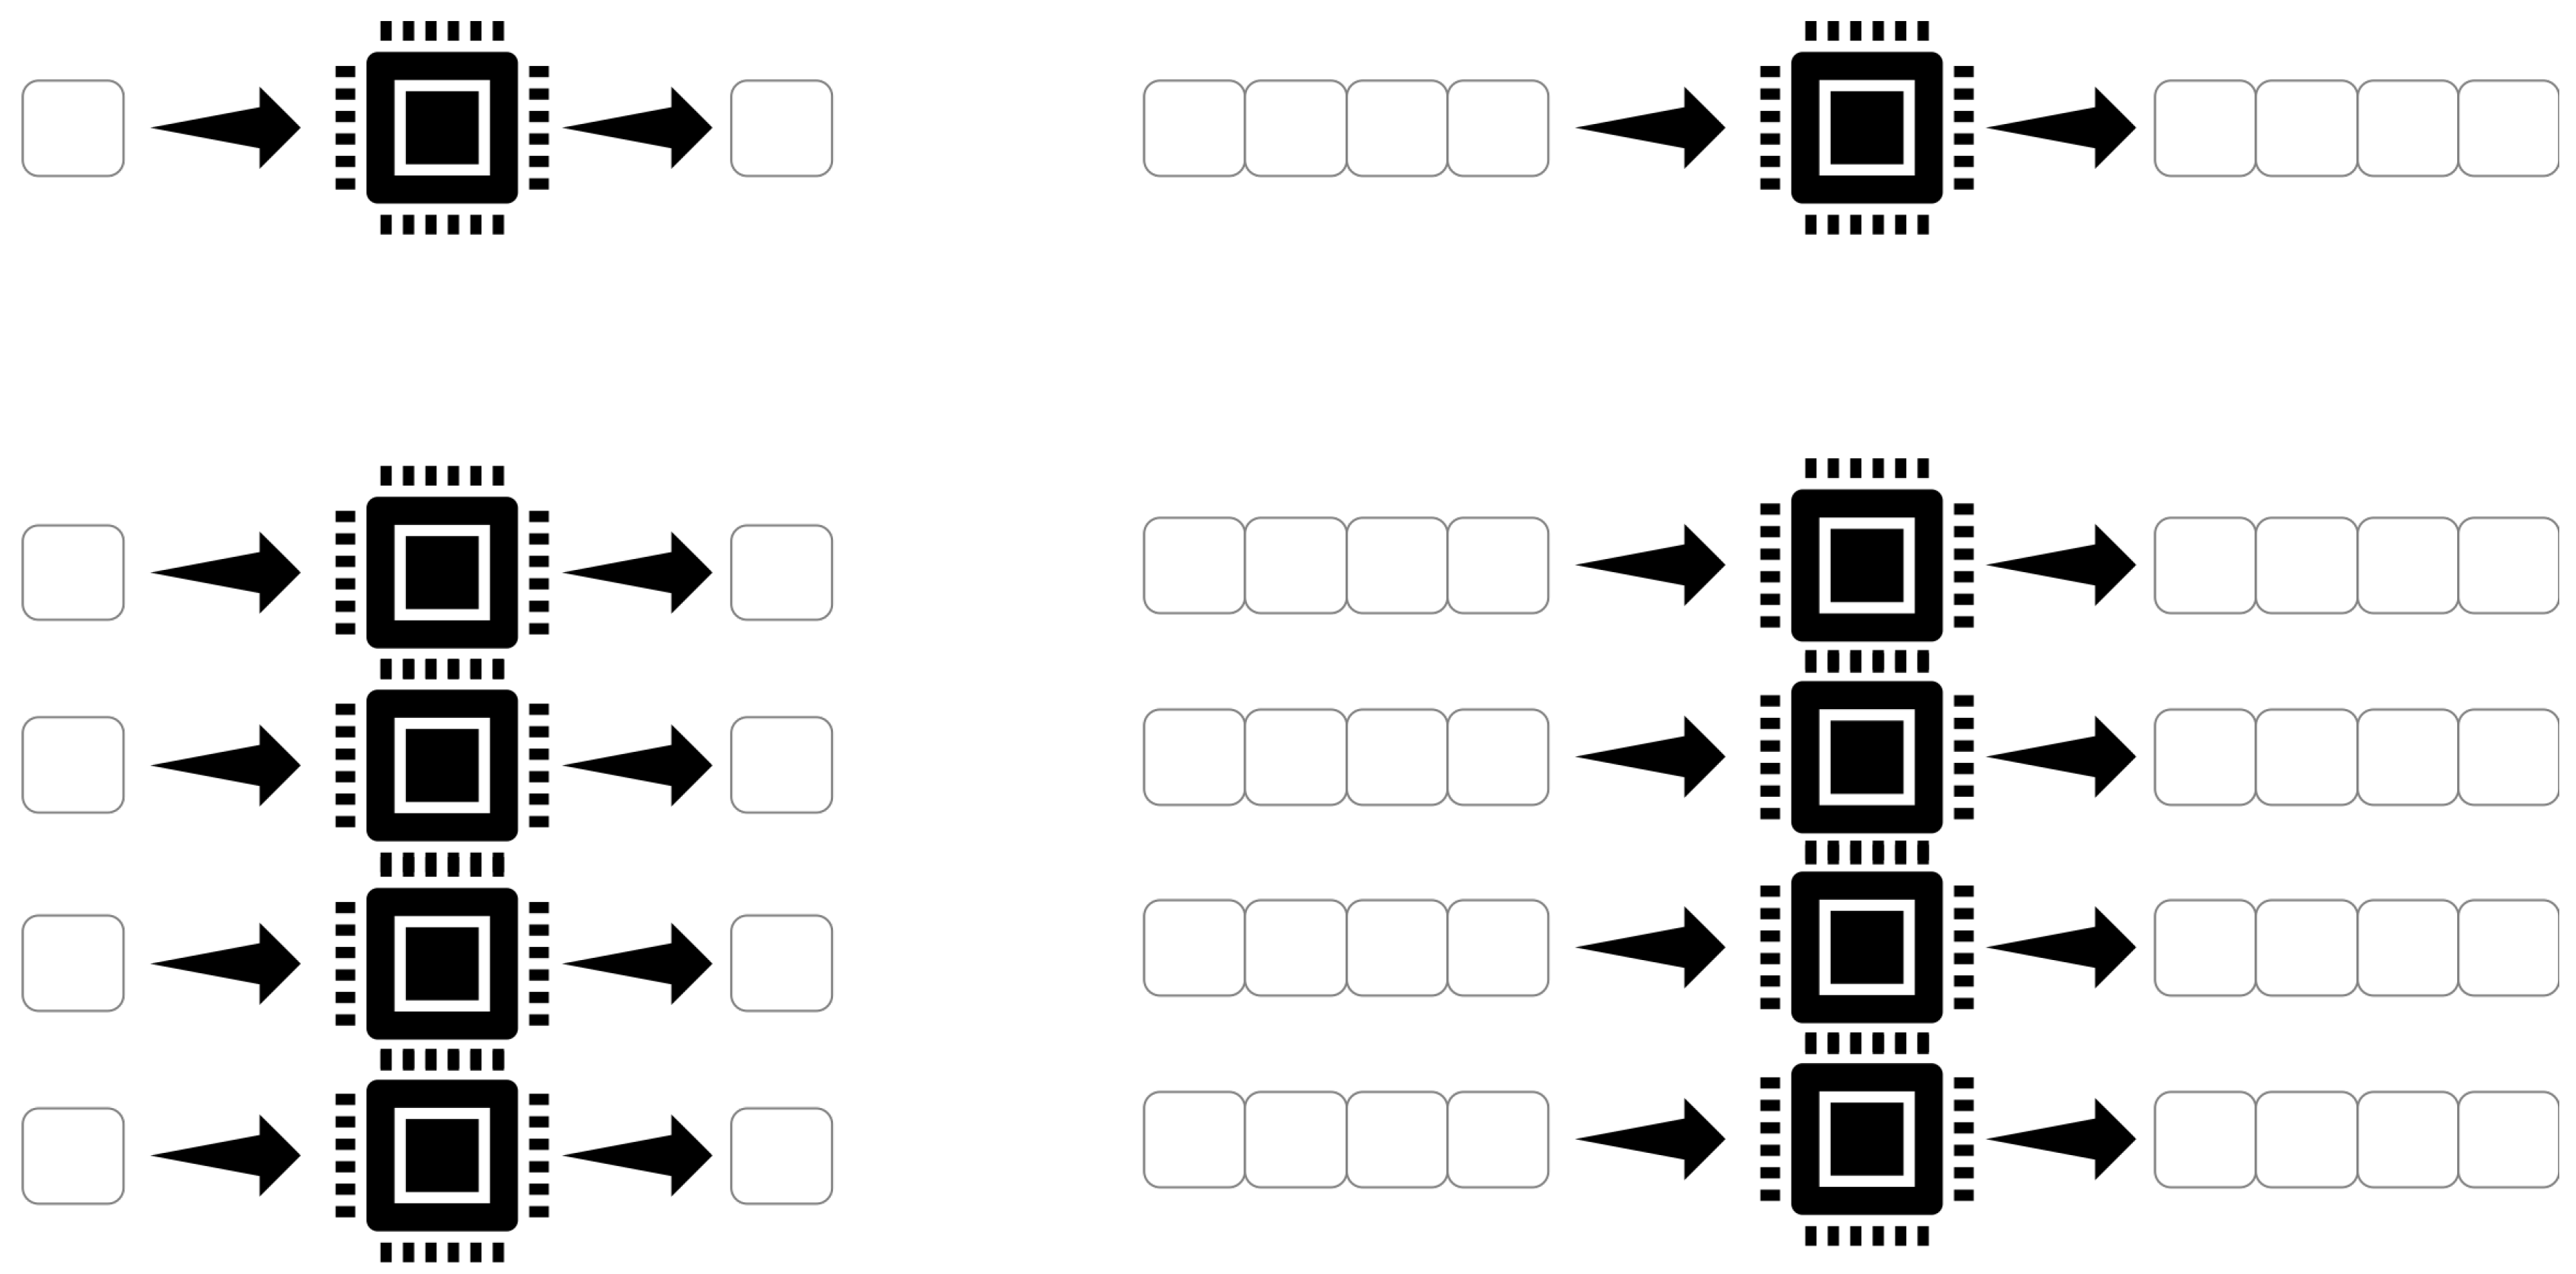
\includegraphics[scale=0.1]{img/ottimizzazioni.png}
        \caption{Confronto tra le varie ottimizzazioni hardware: Baseline (in alto a sinistra), Multicore (in basso a sinistra),
        SIMD (in alto a destra), SIMD Multicore (in basso a destra)}
    \end{center}
\end{figure}

\subsubsection{OpenMP e TBB}

OpenMP e TBB sono due librerie che in fase di sperimentazione sono state utilizzate per testare il parallelismo
\emph{thread-level} in modo da sfruttare i multipli core disponibili nelle moderne CPU. Le due librerie --- poiché
forniscono lo stesso tipo di funzionalità --- sono da utilizzare in modo mutuamente esclusivo. La scelta della 
libreria da utilizzare cadrà dunque su quella che garantisca le migliori prestazioni.

\subsubsection{SIMD}

SIMD (\textit{Single Instruction Multiple Data}) è una classe di istruzioni che consente di ottenere parallelismo su un
singolo core. Il modello prevede l'esecuzione della stessa operazione su una molteplicità di dati mediante l'utilizzo di una
singola istruzione. All'interno di un'istruzione vengono quindi inglobati diversi dati e, ovviamente, l'operazione da svolgersi.

I processori ARM, montati sulla stragrande maggioranza di dispositivi Android così come anche sui modelli di Raspberry Pi già 
testati, dispongono di un'architettura SIMD avanzata chiamata NEON.\\%citazione a qualche documentazione NEON?
Poiché la libreria OpenCV fornisce nativamente supporto per le istruzioni NEON, risulta piuttosto immediato testare l'utilizzo di
tali istruzioni nell'applicazione OTV.
%L'esecuzione fisica di queste istruzioni avviene mediante un'unica unità di controllo che piloti diverse ALU in maniera sincrona,
%ciascuna di queste operanti su un differente dato tra quelli specificati.

L'utilizzo delle istruzioni SIMD può beneficiare specialmente i casi in cui una singola operazione debba essere ripetuta molte
volte su un insieme di dati anche grande. È il caso dell'elaborazione di immagini, in cui spesso è richiesto operare su dati sotto
forma di matrici ed eseguire operazioni anche semplici ma molto ripetitive.

\subsubsection{GPU e OpenCL}

L'utilizzo della potenza di calcolo di una GPU è giustamente considerato tra le ottimizzazioni da testare: qui il parallelismo
è intrinseco al tipo di processore, che è progettato appositamente per svolgere operazioni semplici ma ripetitive su un grande
insieme di dati, in particolare nei casi di elaborazione di immagini. Tuttavia, come evidenziato in \cite{rs12122047}
il potenziale guadagno in efficienza che questa soluzione garantirebbe non è facilmente stimabile e dipende da una varietà di
fattori.

La libreria OpenCL permette di sfruttare le funzionalità della GPU, qualora supportata dal dispositivo in questione.


%\clearpage{\pagestyle{empty}\cleardoublepage}

%===========

%\shipout\null
%\stepcounter{page}

\chapter{Processo di sviluppo}

Parlando ora dell'effettiva operazione di porting di OTV su dispositivo Android, si espongono gli strumenti utilizzati
e le complessità riscontrate durante il processo di sviluppo. Verranno trattati inoltre i dettagli tecnici dell'applicazione
e i meccanismi utilizzati propri del sistema Android.

\section{OpenCV}

Come brevemente spiegato nel capitolo precedente, il codice disponibile di OTV è basato su OpenCV.
Nel caso di Android, i moduli di OpenCV devono essere necessariamente incapsulati all'interno dell'applicazione, non essendo
possibile installarli tra le librerie di sistema. Chiaramente, i moduli dovranno essere compilati con la toolchain di Android
per poter ottenere binari effettivamente compatibili con il sistema operativo.

I binari di OpenCV sono reperibili sul sito ufficiale oppure compilabili manualmente tramite una
\textbf{cross-compilazione}: questa seconda opzione è preferibile in quanto consente di configurare a proprio piacimento
l'installazione di OpenCV, aggiungendo o rimuovendo selettivamente le ottimizzazioni introdotte in \autoref{sec:ottim}.

Tutte le ottimizzazioni hardware discusse, infatti, sono disponibili su OpenCV. 
Non avrebbe senso invece implementarle nel codice OTV poiché tutte le operazioni che facciano uso intensivo della CPU e 
che richiedano tempi di esecuzione piuttosto lunghi sono interne alla libreria OpenCV.
L'unica ottimizzazione che effettivamente viene implementata nel codice di OTV è l'elaborazione delle immagini in scala di
grigi (non essendo a livello hardware): è sufficiente aggiungere una riga di codice nel momento in cui i frame estratti vengono
letti dall'applicazione.

\subsection{Cross-compilazione}

Dovendo testare numerose configurazioni diverse, per la cross-compilazione di OpenCV è stato preparato un semplice script 
in bash che automatizzasse in minima parte il processo e fornisse inoltre uno scheletro da seguire nel caso in cui si 
volesse modificare la configurazione di OpenCV, in particolare aggiungendo o rimuovendo ottimizzazioni hardware. 
Si riporta di seguito il passaggio principale dello script:

\definecolor{bg}{rgb}{0.9,0.9,0.9}

\usemintedstyle{tango}
\begin{minted}[
    frame=lines,
    framesep=2mm,
    baselinestretch=1.2,
    bgcolor=bg,
    fontsize=\footnotesize
]{bash}
    for ABI in "armeabi-v7a" "arm64-v8a"; do
        mkdir -p build_$ABI
        cd build_$ABI
        rm CMakeCache.txt
        cmake \
        -DCMAKE_TOOLCHAIN_FILE=$ANDROID_TOOLCHAIN_PATH \
        -DANDROID_ABI=$ABI \
        -DANDROID_NATIVE_API_LEVEL=$ANDROID_API_LEVEL \
        -DANDROID_STL=c++_shared \
        -GNinja -DCMAKE_BUILD_TYPE:STRING=Release \
        -DBUILD_FAT_JAVA_LIB=OFF \
        -DBUILD_JAVA=OFF \
        -DBUILD_SHARED_LIBS=ON \
        -DWITH_TBB=ON -DBUILD_TBB=ON \
        -DENABLE_NEON=OFF \
        -DWITH_OPENMP=OFF \
        -DWITH_OPENCL=OFF \
        -DWITH_CAROTENE=OFF \
        -DWITH_PTHREADS_PF=OFF \
        -DANDROID_SDK_ROOT=$ANDROID_SDK_ROOT \
        -DANDROID_NDK=$ANDROID_NDK \
        -DOPENCV_ENABLE_NONFREE=ON \
        -DBUILD_TESTS=FALSE -DBUILD_PERF_TESTS=FALSE \
        -DBUILD_ANDROID_EXAMPLES=FALSE \
        -DBUILD_DOCS:BOOL=OFF -DWITH_IPP=OFF -DWITH_MSMF=OFF \
        ..
    
        ninja
        ninja install
        cd ..
    done
\end{minted}

In questo caso viene utilizzato \textbf{CMake} per configurare la compilazione (scelta obbligata, poiché il file CMake è fornito 
nella distribuzione di OpenCV) e \textbf{ninja} come \textit{build system}. 
CMake infatti non esegue la vera e propria compilazione, ma prepara l'ambiente e crea i file di compilazione che 
verranno poi usati dal build system per effettivamente compilare il progetto. In alternativa a ninja era possibile 
utilizzare \textbf{Make}, la scelta fra i due non comporta nessuna differenza nel risultato ma può influire leggermente 
sui tempi di compilazione.

Tra le diverse opzioni di CMake si nota intanto \texttt{ANDROID\_ABI}, che specifica l'ABI per il quale compilare OpenCV. 
Un ABI (\textit{Application Binary Interface}) rappresenta, tra le altre cose, l'insieme di set di istruzioni
supportati da un dispositivo, come spiegato in \cite{adev_abi}. 
Si limita la scelta ad \texttt{armeabi-v7a} e \texttt{arm64-v8a}, rispettivamente le ABI delle architetture ARM a 32 e 64 bit. 
Architetture differenti da ARM non verrebbero comunque testate su Android.

Altre opzioni interessanti sono quelle riguardanti le ottimizzazioni hardware: ad esempio \texttt{WITH\_TBB}, 
\texttt{ENABLE\_NEON} o \texttt{WITH\_OPENCL}. Per abilitare le ottimizzazioni è sufficiente settare a \texttt{ON}
l'opzione di interesse.

\subsection{Installazione}

Una volta ottenuti i binari di tutti i moduli necessari di OpenCV (tramite cross-compilazione o download), è possibile
procedere con l'inserimento all'interno del progetto di Android Studio: come già detto, queste librerie dovranno essere 
parte integrante dell'applicazione.

L'inserimento è molto meccanico e avviene con la creazione di due cartelle nel progetto: una per contenere gli header di
OpenCV, l'altra per contenere le librerie dinamiche contenenti il codice (file \texttt{.so}).
Sia gli header che le librerie vengono inclusi nel progetto aggiungendo istruzioni ad hoc all'interno del file 
\texttt{CMakeLists.txt} generato automaticamente da Android Studio per compilare la componente nativa del progetto che
comunichi con gli entry point Java.
Segue un esempio con le principali istruzioni CMake utilizzate per aggiungere le librerie di OpenCV:

\usemintedstyle{vs}
\begin{minted}[
    frame=lines,
    framesep=2mm,
    baselinestretch=1.2,
    bgcolor=bg,
    fontsize=\footnotesize
]{cmake}

include_directories(${CMAKE_SOURCE_DIR}/../jniIncludes)

add_library( libopencv_core SHARED IMPORTED )
set_target_properties( libopencv_core PROPERTIES IMPORTED_LOCATION
        ${CMAKE_SOURCE_DIR}/../cmakeLibs/${ANDROID_ABI}/libopencv_core.so)

#...

target_link_libraries( 
        # Specifies the target library.
            native-lib

        # Links the target library to the log library
        # included in the NDK.
        ${log-lib}

        libopencv_core
        #...
)

#...
\end{minted}

\section{Sviluppo dell'applicazione Android}

Il deployment e l'installazione di applicazioni su dispositivi Android avviene mediante l'uso di file .APK.
I file APK sono sostanzialmente degli archivi compressi in formato .ZIP il cui contenuto è quindi visualizzabile con
un qualsiasi gestore di archivi. Contengono tutti i file necessari per una singola applicazione Android: librerie native,
classi Java compilate, ma anche risorse e immagini.

La creazione dei file APK a partire dai file sorgente e dal progetto iniziale spetta solitamente a sistemi di compilazione.
Per facilitare questa operazione, viene di norma utilizzato un ambiente di sviluppo e quindi un IDE specializzato.\\
Nel caso di Android l'IDE consigliato è Android Studio, che fornisce un bundle di installazione contenente tutti gli strumenti
e le toolchain necessarie, facilmente configurabili.

Il linguaggio principale supportato da Android è \textbf{Java} (ultimamente anche Kotlin sta avendo largo impiego): 
ogni applicazione richiede anche solo una minima parte scritta in Java o Kotlin per poter utilizzare le API di sistema e gestire i 
cosiddetti \emph{Entry Point} dell'applicazione, ovvero i meccanismi tramite i quali l'utente può avviare ed interagire con 
l'applicazione, l'interfaccia utente è infatti manipolabile esclusivamente con l'utilizzo di classi Java/Kotlin.

È comunque disponibile il supporto per codice nativo C/C++ grazie all'NDK (\emph{Native Development Kit}): un insieme di strumenti
per la compilazione e il debug integrabili con Android Studio. Lo strumento di configurazione di default per codice nativo è 
CMake, tra i più diffusi per progetti C e C++: un esempio di configurazione tramite CMake è quello giusto esposto nella
sezione di cui sopra, in cui si aggiungono le librerie OpenCV al progetto.

Per configurare infine il progetto nella sua interezza, compresi i dettagli di deployment, Android Studio richiede l'utilizzo 
del plugin \textbf{Gradle}, che può essere integrato con CMake (in modo molto automatizzato) qualora sia prevista la 
presenza di codice nativo.

\subsection{Architettura dell'applicazione}

Il codice Java e quello nativo, all'interno di un'applicazione Android, comunicano grazie al framework \textbf{JNI} 
(\textit{Java Native Interface}). Questo framework consente in modo particolare l'invocazione di funzioni scritte in codice
nativo da parte di classi Java. 

Nonostante il funzionamento di JNI sia piuttosto complesso (si veda la documentazione in \cite{jnispec}), l'utilizzo di esso 
in un progetto Android Studio avviene in modo piuttosto guidato e trasparente nei confronti dello sviluppatore: tutti i 
dettagli interni di collegamento e configurazione tra i vari componenti vengono gestiti in maniera automatizzata. 
Inoltre, come si vedrà, ai fini di questo progetto è stato sufficiente fare uso delle funzioni più basilari di JNI.

Dopo un'attenta analisi, si è deciso di strutturare l'applicazione come segue:
\begin{itemize}
    \item Entry point Java (\texttt{MainActivity.java});
    \item Classe Java che implementi un \emph{thread} secondario per l'invocazione del codice OTV (\texttt{OTVThread.java});
    \item File C++ che faccia da wrapper per le funzionalità di OTV, interfacciandosi con il codice Java (file 
    \texttt{native-lib.cpp});
    \item Codice di OTV, pressoché inalterato (cartella \texttt{otv/src/}).
\end{itemize}

Il motivo per cui si è scelto di introdurre un thread apposito per l'invocazione di OTV è legato alle modalità con cui la 
classe MainActivity gestisce l'interazione con l'utente.
Ogni \textit{Activity} ha un ciclo di vita --- descritto in \cite{adev_lifecycle} --- basato su funzioni di callback invocate dal sistema
Android a seguito di determinate azioni compiute dall'utente, ad esempio il metodo \texttt{onCreate}, invocato non appena
l'utente apre l'applicazione.

Poiché OTV presenta le caratteristiche di un demone (ha un ciclo di esecuzione che idealmente non termina mai), inserirlo 
all'interno di un metodo di callback significherebbe deviare dal normale ciclo di esecuzione dell'attività.
La scelta di un thread che esegua OTV in background è quasi obbligata in quanto è l'unico modo di garantire un'esecuzione
(quasi) disaccoppiata dagli eventi della UI ma soprattutto che avvenga in modo asincrono rispetto alla creazione degli elementi
dell'interfaccia grafica: se si invocasse OTV all'interno del metodo \texttt{onCreate}, l'applicazione risulterebbe bloccata 
sulla creazione dell'interfaccia.

Nel metodo \texttt{onCreate} della classe \texttt{MainActivity} risulterà quindi:

\usemintedstyle{vs}
\begin{minted}[
    baselinestretch=1.2,
    fontsize=\footnotesize
]{java}
protected void onCreate(Bundle savedInstanceState) {
    //...
    OTVThread otvThread = new OTVThread(updateUIHandler);
    otvThread.start();

    //casella di testo nella UI
    tv.setText("OTV was launched in background...");
}
\end{minted}

Nella classe \texttt{OTVThread}:

\usemintedstyle{vs}
\begin{minted}[
    baselinestretch=1.2,
    fontsize=\footnotesize
]{java}
public void run() {
    String otv_results = runOTV();
    //...
}

// metodo nativo invocabile tramite JNI
public native String runOTV();
\end{minted}

\vspace{1em}

Infine, nel wrapper C++ (\texttt{native-lib.cpp}):

\vspace{1em}

\usemintedstyle{vs}
\begin{minted}[
    baselinestretch=1.2,
    fontsize=\footnotesize
]{cpp}

extern "C" JNIEXPORT jstring JNICALL 
Java_gullp_androidotv_OTVThread_runOTV( JNIEnv* env, jobject) {

    //costruzione dei parametri richiesti
    char* argv[6];
    argv[0] = "OTV_AndroidInstance";
    argv[1] = PATH_INFO_VIDEO;
    argv[2] = PATH_FILE_PARAMS;
    argv[3] = PATH_LK_FILE;
    argv[4] = PATH_OUTPUT;
    argv[5] = PATH_MASK;

    LOGD("Running OTV...");

    //effettiva invocazione del codice OTV nativo
    return env->NewStringUTF(run(6, argv).c_str());
}

\end{minted}

\vspace{1em}

I file di configurazione richiesti da OTV (contenenti i parametri di calibrazione per l'algoritmo di Lucas Kanade)
sono stati inseriti nella cartella \texttt{/data/data/\{nome\_package\}} del dispositivo, che rappresenta la porzione di 
storage interno dedicata all'applicazione.

%===========

\chapter{Test e risultati}

Completato lo sviluppo dell'applicazione, ha avuto luogo la fase finale nonché probabilmente la più importante: il testing 
di varie configurazioni e la conseguente raccolta ed analisi dei risultati, al fine di valutare i vantaggi e gli svantaggi di 
un porting sul sistema Android.

A differenza del testing su Raspberry Pi, i cui modelli sono molto standardizzati e distribuiti dallo stesso produttore,
per gli smartphone Android i risultati ottenuti in termini di performance e consumi possono variare anche molto al variare
del dispositivo, a seconda delle caratteristiche tecniche di quest'ultimo.

Per quanto riguarda il seguente progetto, i test sono stati svolti su un dispositivo Android basato sul 
SoC \textit{Qualcomm Snapdragon 730} (sul quale è presente una CPU octa-core).\\
Sono quindi prevedibili risultati 
migliori (perlomeno in termini di prestazioni) rispetto a dispositivi aventi caratteristiche tecniche inferiori.

\section{Testing}

Ai fini del testing sono stati utilizzati fotogrammi precedentemente estratti poiché riprodurre l'intero processo
di acquisizione ed estrazione andrebbe oltre gli scopi limitati del seguente lavoro e aggiungerebbe notevole complessità 
al progetto, costringendo a fare i conti con diversi problemi (ad esempio, la mancanza di \textit{ffmpeg} su Android).
Difatti, nel testare l'applicazione si è considerata esclusivamente la fase di esecuzione, tralasciando le altre tre fasi
presentate in \autoref{sec:ciclo} principalmente per motivi di tempo. L'esecuzione di OTV rappresenta comunque la fase più
importante e con il maggior numero di variabili che possano influenzare le prestazioni e i consumi: le analisi che ne
conseguono sono sicuramente indicative delle potenzialità di un dispositivo.

Il testing è stato eseguito mediante l'ausilio degli strumenti forniti dalla repository GitHub di OTV (\cite{otvgit}),
in particolare gli script Bash adibiti alla creazione dei file di configurazione richiesti per il funzionamento del programma.
Lo script che implementa l'estrazione dei frame a partire da un file video fa uso del programma
\textit{ffmpeg} e salva i fotogrammi estratti all'interno di una cartella \texttt{frames} il cui percorso va specificato.

La cartella dei frames e gli altri file necessari sono stati quindi prima generati sulla macchina utilizzata per lo sviluppo
dell'applicazione, poi trasferiti sul dispositivo Android mediante l'interfaccia grafica fornita da Android Studio.
Collegando infatti lo smartphone al PC su cui esegue Android Studio è possibile accedere ad una sezione dedicata al file system
del dispositivo.

Come già menzionato, tutti i file di servizio sono stati inseriti all'interno della cartella \texttt{/data/data/\{package\_applicazione\}}
poiché questa fa parte del cosiddetto storage \emph{interno} dell'applicazione, in cui gli accessi non sono vincolati da permessi
richiesti all'utente. Questa cartella inoltre non è accessibile dall'utente se non tramite strumenti esterni al dispositivo 
(come il debugger Android) e può quindi essere utile ad evitare cancellazioni e/o modifiche accidentali dei file necessari.

Particolare attenzione va posta al file \texttt{info\_video.txt}, generato in seguito all'estrazione dei frame. Il file si
presenta nel seguente modo:

\begin{verbatim}
    FPS 25
    Width 715
    Height 540
    FileCount 500
    DirectoryFrame /data/data/gullp.androidotv/frames
    Jump 2
\end{verbatim}

dove il parametro DirectoryFrame rappresenta la directory in cui sono presenti i frame: il file viene letto dall'applicazione
in fase di inizializzazione, quindi è importante che il percorso di tale directory sia accurato.
Tuttavia, essendo il file \texttt{info\_video.txt} generato da uno script eseguito su una macchina differente, è necessario
andare a modificare tale parametro specificando la corrispettiva cartella nel dispositivo Android.

\vspace{1em}

Il processo di testing è avvenuto seguendo un'iterazione di questo tipo:

\begin{enumerate}
    \item Copia delle librerie dinamiche precompilate di OpenCV all'interno del progetto, ottenute con la cross-compilazione 
    e nelle quali è attivo uno specifico set di ottimizzazioni;
    \item Esecuzione dell'applicazione e trascrizione dei risultati ottenuti
    \item Ripetizione del punto 2 fino ad ottenere una quantità soddisfacente di risultati
    \item Reiterazione a partire dal punto 1 utilizzando una nuova configurazione di OpenCV
\end{enumerate}

\vspace{1em}

I risultati così ottenuti sono poi stati sottoposti ad un'analisi finale per stabilire i vantaggi di ciascuna configurazione. 

\section{Stima dei consumi energetici}

Data l'influenza che i consumi energetici hanno sulla realizzabilità e sulla valutazione di un dispositivo embedded di questo
tipo, si è deciso di svolgere --- anche se non approfonditamente --- una stima dell'energia consumata da esso.
È importante notare che si tratta di una stima, poiché gli strumenti utilizzati consentono un livello di precisione piuttosto
basso nella misurazione dei consumi su periodi piuttosto brevi di tempo.

Per stimare i consumi energetici dell'esecuzione di OTV è stato utilizzato uno strumento messo a disposizione per gli 
sviluppatori Android: \textit{\textbf{Battery Historian}}. Si tratta di un tool web il cui utilizzo molto semplice è 
descritto in \cite{adev_battery}. In sostanza, analizza i file di log generati dal dispositivo e ne visualizza gli eventi
correlati al consumo di batteria, fornendone una presentazione ad alto livello tramite grafici e tabelle.
Tra i parametri analizzati da Battery Historian figurano il livello di carica della batteria (in $mAh$) e la tensione generata
da essa (in $V$). L'analisi viene svolta su tutto l'arco temporale coperto dai log: è bene quindi resettare i log relativi
all'uso della batteria.

I file di log necessari all'utilizzo di Battery Historian possono essere acquisiti mediante il debugger Android (\texttt{adb}): 
la procedura guidata è disponibile in \cite{adev_batlog}.

\begin{figure}[h!]
    \begin{center}
        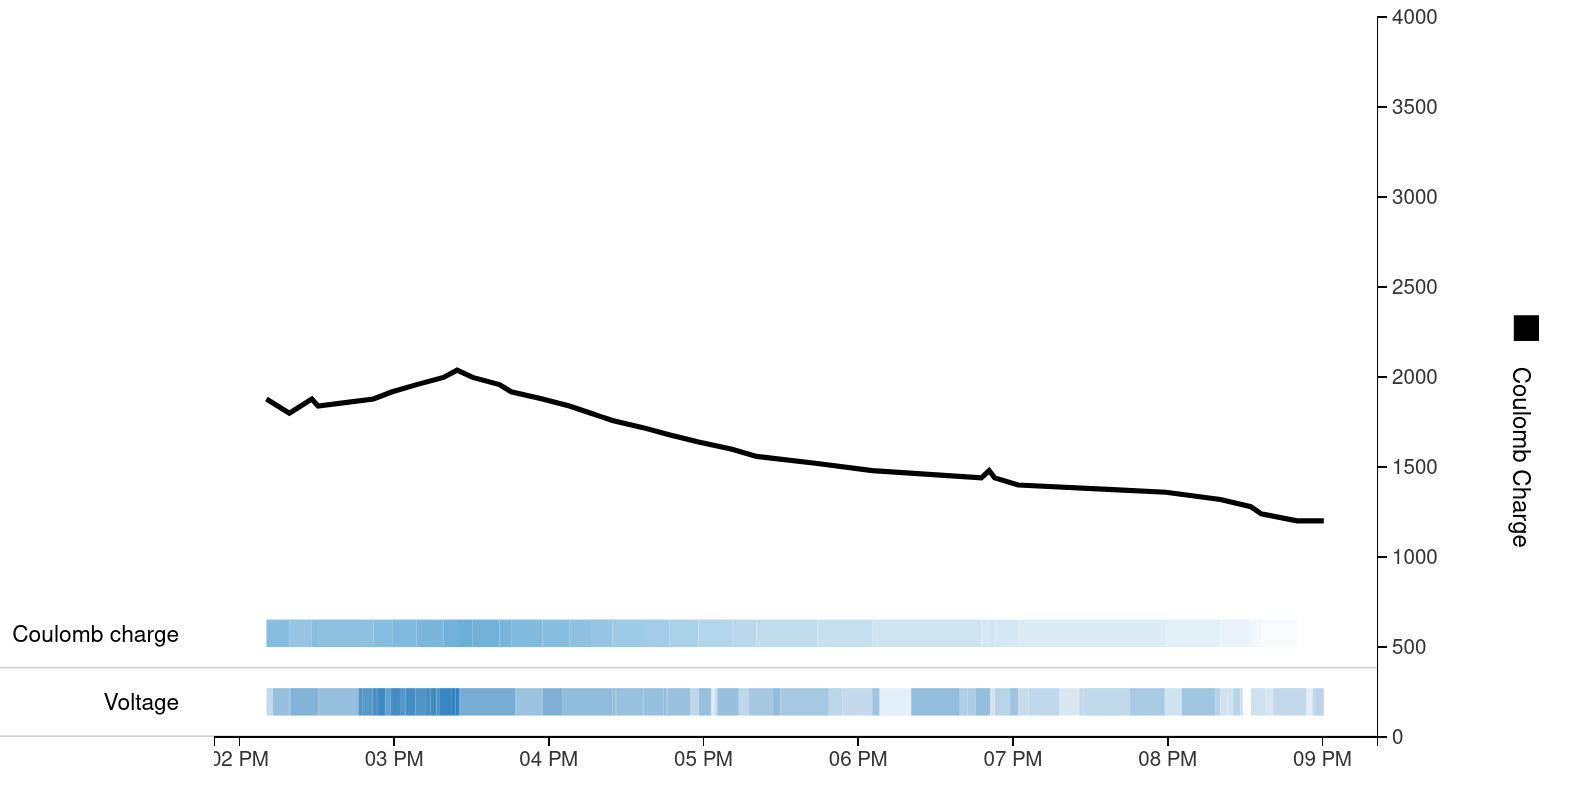
\includegraphics[scale=0.38]{img/battery_historian_coulomb.png}
        \caption{Andamento nel tempo del livello di carica della batteria in $mAh$}
    \end{center}
\end{figure}

L'immagine di cui sopra rappresenta uno dei grafici ottenibili con Battery Historian di maggiore interesse al fine di
determinare il consumo energetico: l'andamento del livello di carica. Passando il cursore lungo il grafico è possibile
ottenere informazioni aggiuntive particolarmente utili:

\begin{figure}[h!]
    \begin{center}
        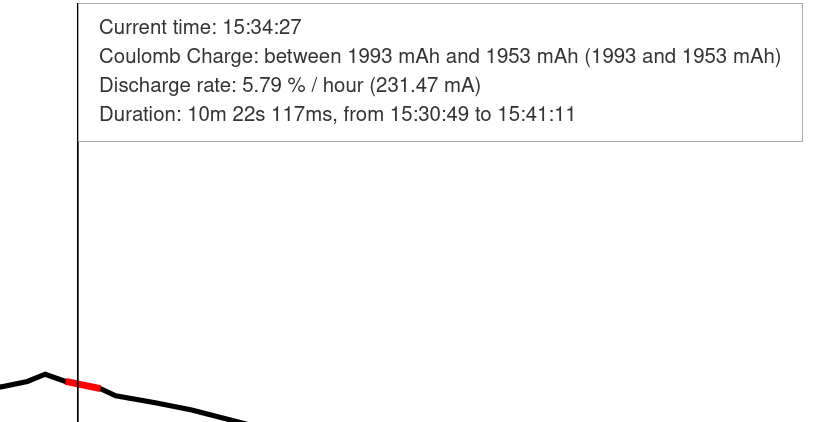
\includegraphics[scale=0.5]{img/battery_historian_hover.png}
        \caption{Informazioni dettagliate relative ad uno specifico intervallo di tempo}
    \end{center}
\end{figure}

Come si può in parte notare dalla figura, l'andamento è discretizzato con dei campionamenti del livello di carica ad 
intervalli di tempo non regolari.

Il dettaglio più interessante tra quelli forniti è il \textit{Discharge rate} espresso in $mA$: è il rapporto tra la differenza
di carica $\Delta Q$ e la lunghezza dell'intervallo $\Delta t$ e rappresenta quindi la media della \textbf{corrente in uscita} 
dalla batteria sull'intervallo di tempo:

\begin{equation*}
    I_{i} = \frac{\Delta Q_i}{\Delta t_i}
\end{equation*}

È possibile comunque applicare la medesima espressione conoscendo la carica in $mAh$ sapendo che $1~mAh = 3.6~C$.

A questo punto, per calcolare la potenza dissipata dallo smartphone durante l'esecuzione di OTV e dunque ottenere l'energia 
consumata, è necessario avere a disposizione altre due informazioni:
\begin{itemize}
    \item I tempi di inizio e fine dell'esecuzione di OTV
    \item Il valore della tensione durante l'esecuzione
\end{itemize}

Entrambe le informazioni sono reperibili immediatamente grazie alle tabelle fornite da Battery Historian.
Analizzando i grafici della tensione si nota che essa non è costante ma soggetta a variazioni molto frequenti, 
tende tuttavia ad assumere valori piuttosto omogenei con una bassa varianza ed è quindi approssimabile ad un valore medio
con una discreta precisione, specie se l'intervallo di tempo analizzato è relativamente piccolo (60 secondi con la configurazione
peggiore di OTV).\\
Supponendo quindi di approssimare la tensione ad un valore $V$ e di avere a disposizione $N$ intervalli di calcolo della
corrente durante l'esecuzione di OTV, è possibile calcolare l'energia consumata basandosi sulla potenza media dissipata come segue:

\begin{equation*}
    %E = P \cdot \Delta t = \sum_{t_i = t_1}^{t_N} V_{t_{i-1}, t_i} \cdot I_{t_{i-1}, t_i} \cdot (t_i - t_{i-1})
   %\\
    E = P \cdot \Delta t = \sum_{i = 1}^{N}~V I_i \cdot \Delta t_i
\end{equation*}

Dove $\Delta t$ è la durata dell'esecuzione di OTV e $\Delta t_i$ è la lunghezza dell'intervallo di tempo in cui
si verifica la corrente i-esima $I_i$.\\
Poiché, come fatto notare poco sopra, l'esecuzione di OTV termina in un lasso di tempo piuttosto breve, sono spesso osservabili
tensioni e correnti costanti lungo tale periodo.

\section{Analisi dei risultati}

Al termine del progetto ha avuto luogo la fase di analisi dei risultati, sia dal punto di vista delle prestazioni che dei 
consumi.

Si riportano di seguito i dati ottenuti in termini di tempo di esecuzione, evidenziando le differenze tra le varie configurazioni.

\ldots

Come si può notare, l'elaborazione in scala di grigi influisce notevolmente sulle prestazioni, dimezzando i tempi nella quasi
totalità dei casi. Sorprendentemente, l'abilitazione di opzioni quali l'uso della GPU con OpenCL e di istruzioni SIMD NEON non
ha influito in alcun modo sull'esecuzione. 

Con molta probabilità, poichè i tempi di esecuzione con e senza tali ottimizzazioni
sono assolutamente inalterati, ciò è dovuto al mancato utilizzo di GPU e istruzioni SIMD o all'utilizzo forzato di queste.
Il motivo più plausibile è che OpenCL non sia completamente supportato dal dispositivo Android in questione. Per quanto riguarda
NEON, è possibile che questo venga utilizzato indipendentemente dalla configurazione scelta.

\ldots

Nel testare i consumi energetici sono state abilitate tutte le possibili ottimizzazioni software fornite dal sistema Android:
disabilitazione di connessione dati, Wi-Fi, Bluetooth e attivazione della \textbf{modalità risparmio energetico}, avendo cura di
mantenere attive le funzionalità basilari necessarie alla comunicazione (es. SMS). Nessuna di queste ottimizzazioni ha 
influito negativamente sulle prestazioni dell'applicazione.

%===========

%\chapter*{Conclusioni}

\chapter*{Conclusioni}
\label{cap:conclusioni}
\addcontentsline{toc}{chapter}{\nameref{cap:conclusioni}}




%\clearpage{\pagestyle{empty}\cleardoublepage}


% --------------- Fine contenuto, inizio bibliografia ---------------

\bibliographystyle{IEEEtran}
\bibliography{refs}

\thispagestyle{empty}

\end{document}